\section{Benchmark results}
Figure 1 shows the time taken to all the elements into a tree (which was pre-populated with 1.000 elements) as the total number of elements in the list grows. Compared are the add time (in red) and the lookup times (in blue)

\begin{figure}
    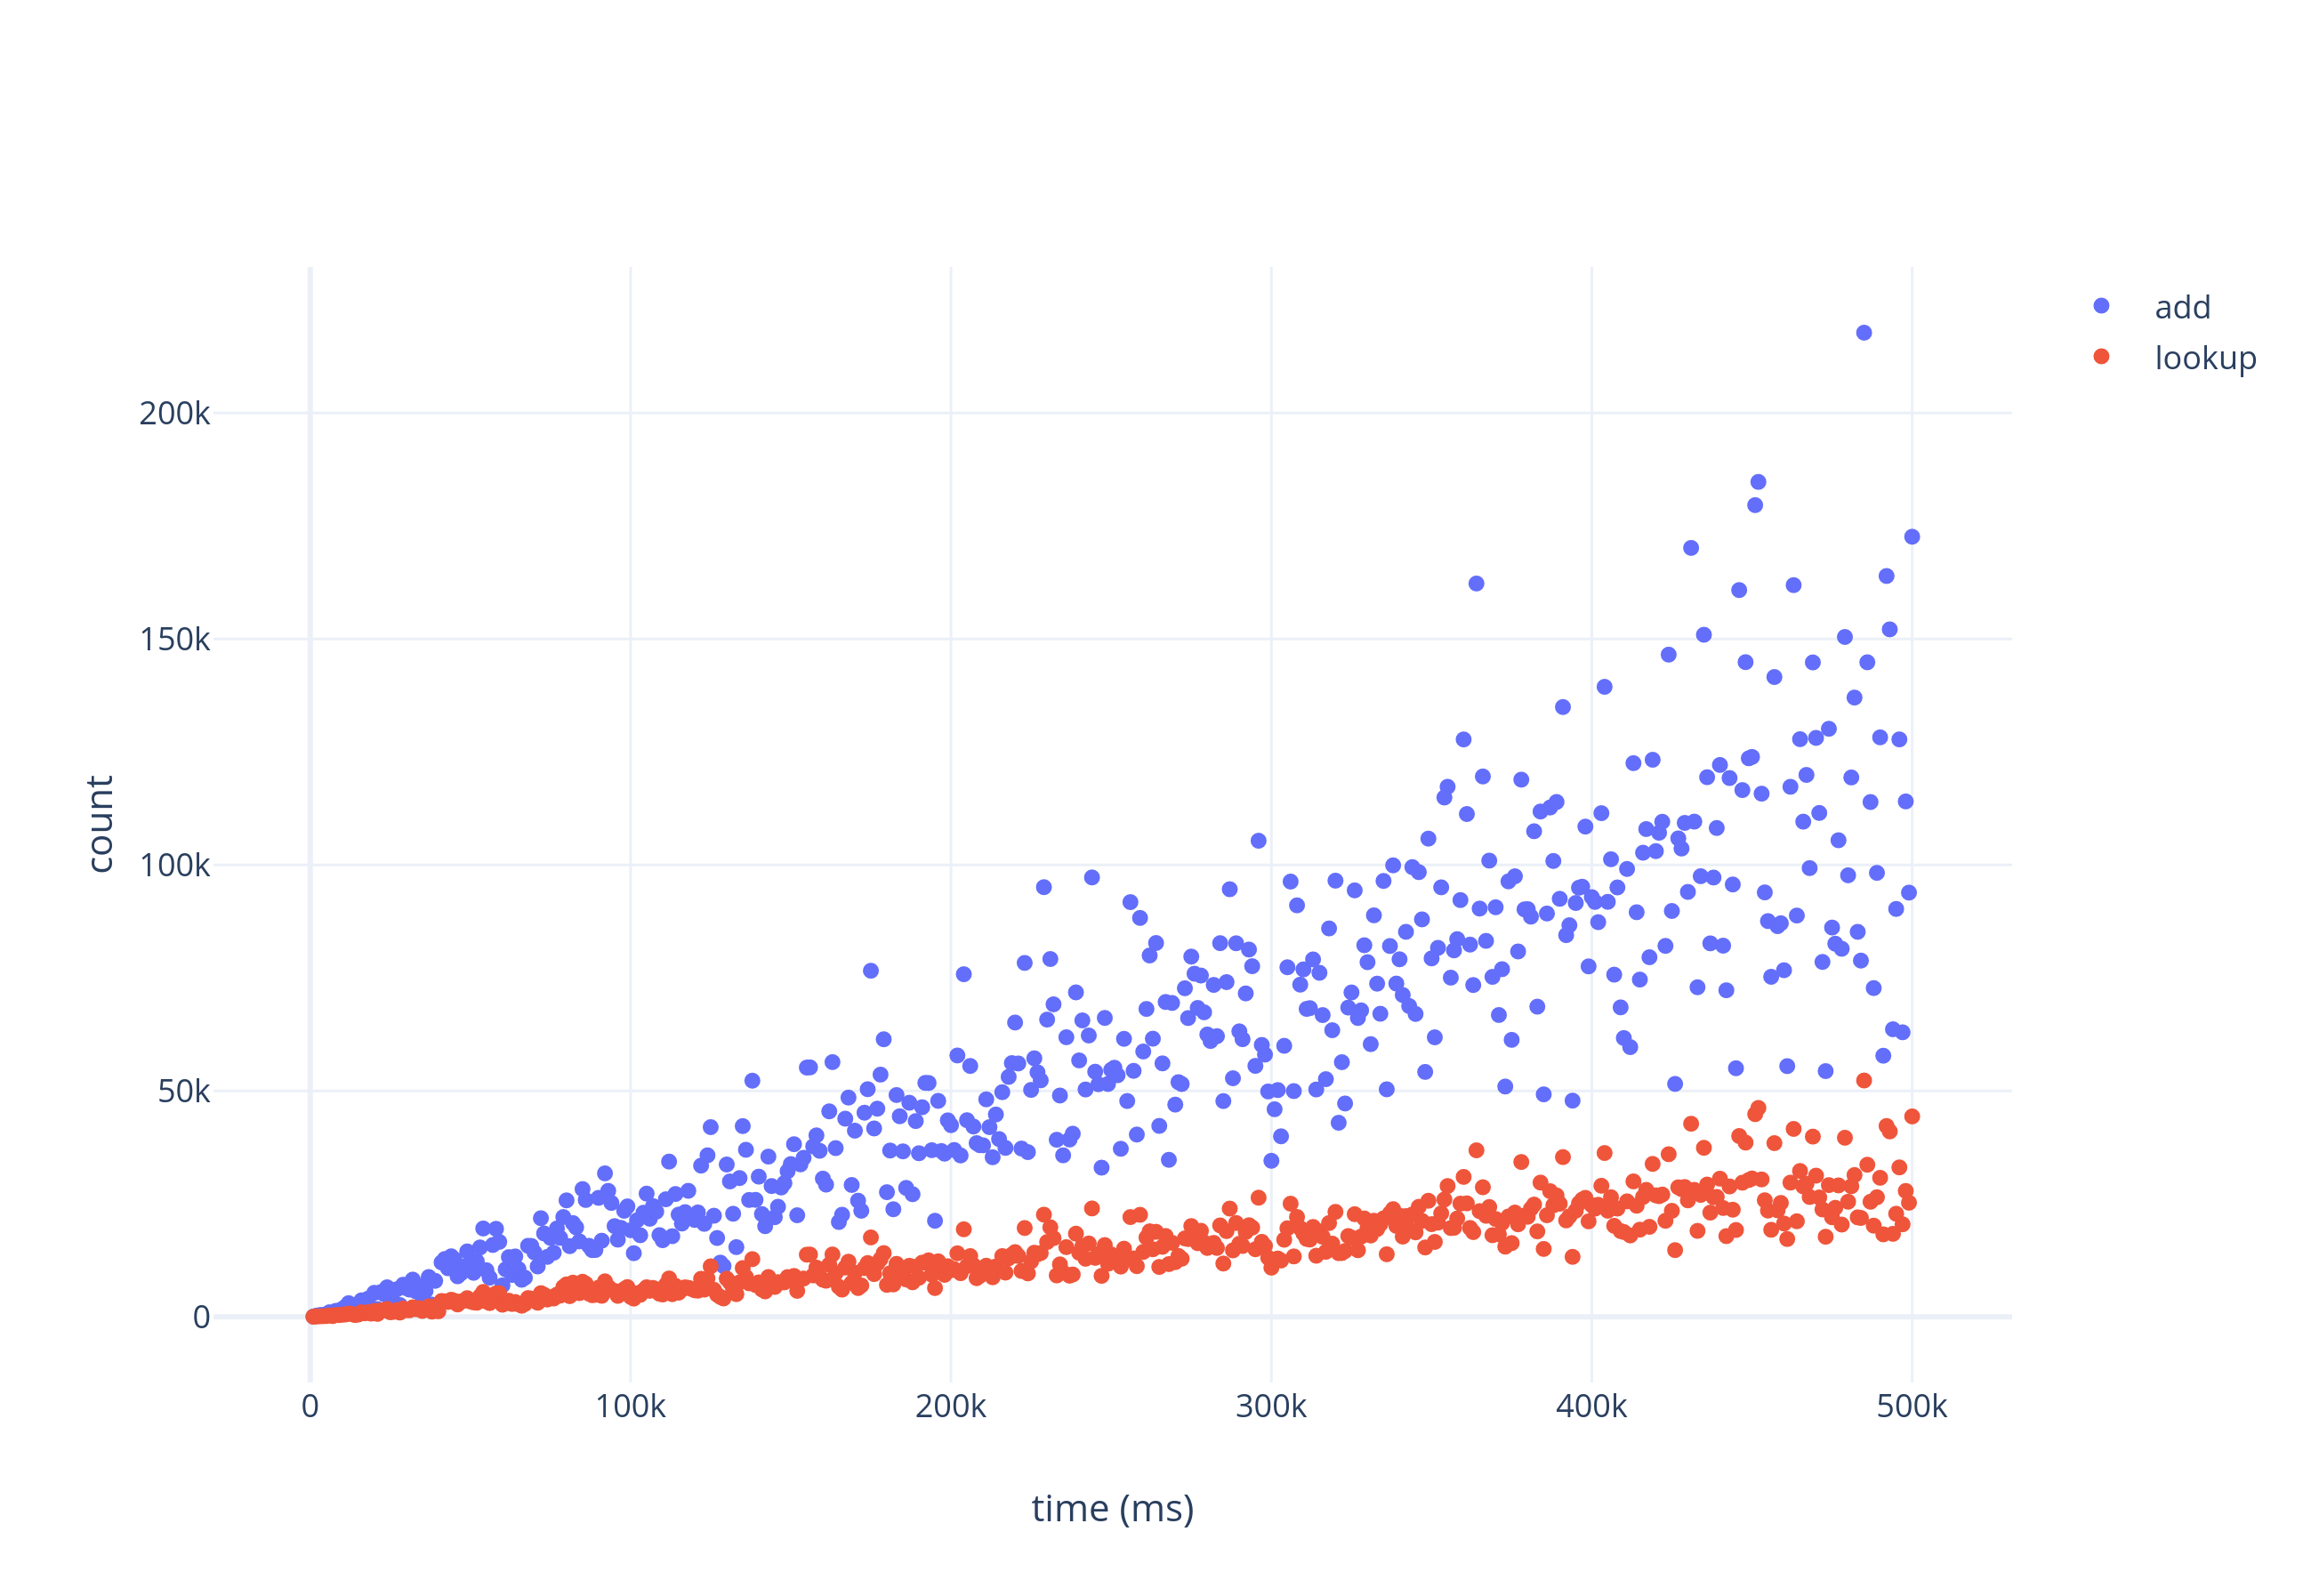
\includegraphics[width=\textwidth]{r_benchmark_non_empty_list}
    \caption{Some caption here}
\end{figure}


As can be seen, the graph looks to be ordo $O(n)$ which is different from a traditional $O(\log n)$ of a binary tree. Two explanations for this: a) the benchmark measures the total time taken for all elements to be added (instead of a single element in each iteration) and b) inefficiencies in Elixir pattern matching which may have influenced our results. 